This section describes the overall design of our system, first with a system overview and then with more in depth information about our tabs.
\subsection{How our web application works}
%figure x5
\begin{figure}[h]
\centering
\includegraphics[width=1\textwidth]{web_system_backboneWebapp.png}
\caption{\label{fig:web_system_backboneWebapp}A general build of a backbone web app.}
\end{figure}

\refer{fig:web_system_backboneWebapp} shows how a backbone\cite{web_1} web application works in general. We have a user that interacts with a browser. A browser renders the DOM\footnote{\textit{Document Object Model}, a convention for representing and interacting with objects in HTML.} of our web application. How it does this is up to the browser. Different browsers might display it differently. Models and Collections will talk to the server to update themselves. For example, our \textit{Experiments} collection will retrieve experiments from the server and update itself with a call to it’s fetch() method. Out of the components that go into this figure, we are in charge of and only capable of changing a few of these; \textbf{View}, \textbf{Template}, \textbf{Collection} and \textbf{Model}. See \textit{Backbone} in section \ref{sec:web_frame} more information.

\subsection{System overview}
%figure 2
\begin{figure}[h]
\centering
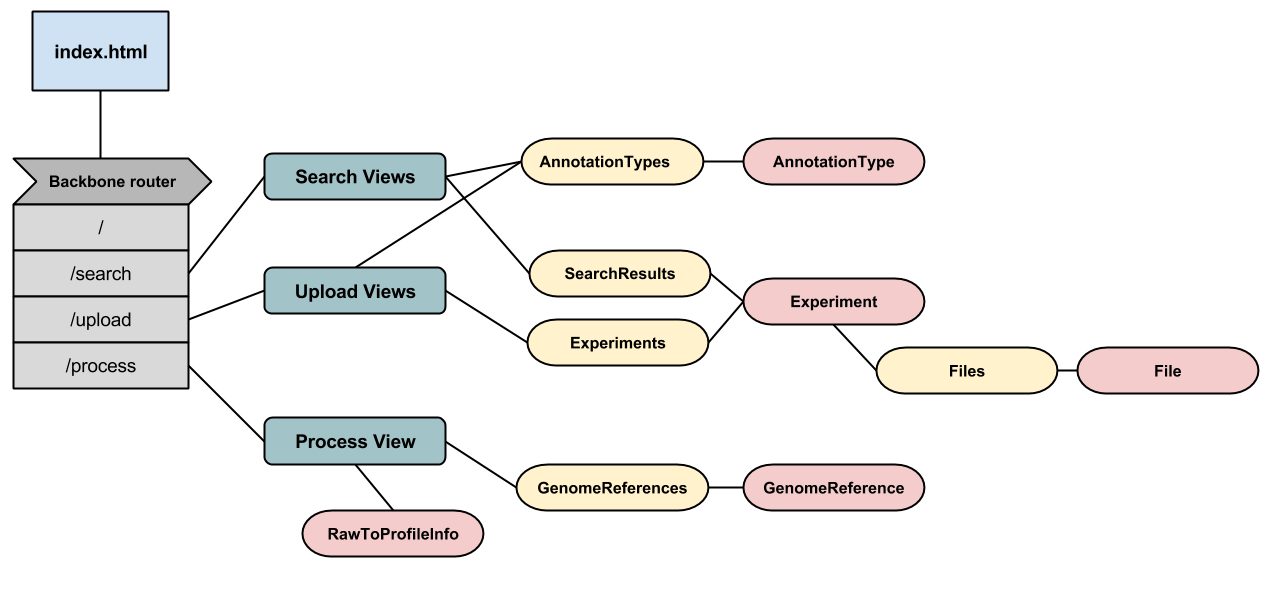
\includegraphics[width=1\textwidth]{web_system_overview.png}
\caption{\label{fig:web_system_overview}Overview of the relations between the different Javascript prototypes in the system.}
\end{figure}

Since our app is built using Backbone\cite{web_1}, our app is divided into the parts \textbf{Misc}, \textbf{Views}, \textbf{Collections} and \textbf{Models}. In \refer{fig:web_system_overview}, we can see the system overview. The \textbf{views} are the parts in green, the \textbf{collections} the parts in yellow and the \textbf{model} the parts in red. For example, the collection \textit{Files} contains a set of \textit{File} models. The model \textit{Experiment} contains a \textit{Files} collection. An \textit{Experiment} model may be used by the collections \textit{SearchResult} and \textit{Experiments}.

The parts in grey represent the router which belongs in our Misc category. It is responsible for rerouting links. For example, when a user clicks the search tab, the router navigates to /search, but instead of loading the whole /search over the page we are currently on, our router will open our search tab below our navigation bar. The \textbf{Misc} category also holds our Main.js, which is in charge of setting up and starting the app. The views are responsible for the user interface, displaying information and handling events. The collections and models are responsible for holding the data.

\label{sec:web_search}
\subsection{Search}
The search tab has three views, that together make up the "Search Views" as we have denoted them in \refer{fig:web_system_overview}. When searching for data, the models and collections will update themselves to contain the new annotations, experiments and files pertaining to that particular search, so the \textit{Search Views} can display them. Once new data has been retrieved, the user can perform a number of actions on the displayed data. For example, when a user chooses to remove a file, the \textit{Search Views} will receive the event, and tell the file's model to destroy itself. The model will then send a delete request to the server, and disappear.

 
%figure bla bla/lalalallala
\begin{figure}[h]
\centering
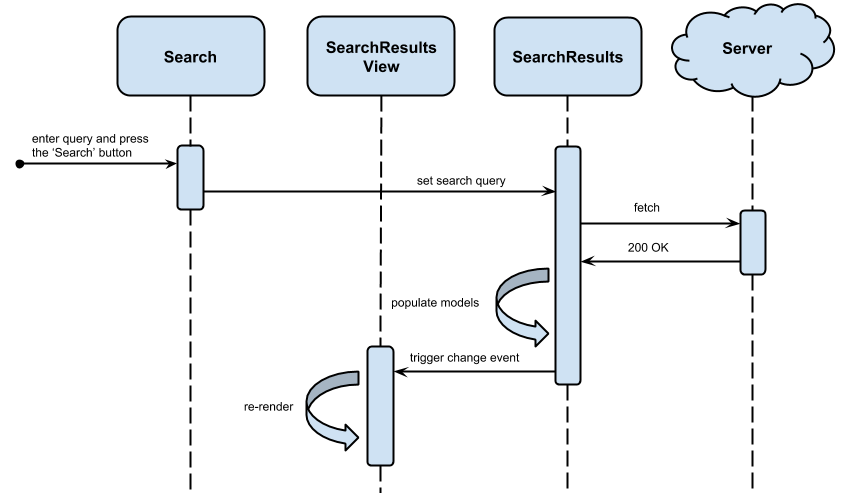
\includegraphics[width=1\textwidth]{web_system_sequenceDiagram.png}
\caption{\label{fig:web_system_sequenceDiagram}a sequence diagram showing what happens when a user enters a valid search query and results are fetched.}
\end{figure}

In \refer{fig:web_system_sequenceDiagram} is a simple sequence diagram for the search tab. If a user enters a query in the search field and then presses the search button, the \textit{Search} view will update the \textit{SearchResults} collection to have a new query. Once \textit{SearchResults} has a new query, it will try to fetch search results corresponding to the query from the server. If successful, new experiment models for every experiment retrieved will be created and set in the \textit{SearchResults} collection. \textit{SearchResults} then triggers a ‘change’ event that \textit{SearchResultsView} listens to. When that event occurs, \textit{SearchResultsView} knows that \textit{SearchResults} has been changed, and re-renders itself.

\subsection{Process}
Process has a single view that is a \textit{modal}, meaning that it is not a full page like the other tabs but a pop-up that appears over the search view when a user chooses an experiment to process. Process has collections and models to store and send data necessary for a process, like genome releases available for the chosen experiment's specie.   

\subsection{Upload}
The upload tab has three views, that together make up the "Upload Views" as we have denoted them in \refer{fig:web_system_overview}. Unlike search (see section \ref{sec:web_frame}) that uses experiment and file models to retrieve information about experiments and files, upload uses the same models to create new experiments and files. To do this, it needs to be aware of what annotations are available, so it uses an annotation type collection to retrieve the current annotations offered when a user wants to create a new experiment.
